%
% Author: Antigoni Kourou
%
\let\textcircled=\pgftextcircled
\chapter{Results}
\label{chap:res}
\initial{S}entiment analysis and feature extraction from text reviews of Airbnb feedback system, provides us a set of discrete estimators for customers' opinions. The sentiment scores can vary from -1 (extremely negative) to 1 (extremely positive). From the analysis of reviews on Amsterdam dataset the most negative sentiment is -0.964284 and the highest score 0.998195. In total there are 12 798 negative sentences (sentiment lower than 0) and 236 904 positive ones, meaning the number of positive sentences is almost 19 times higher. This can be clearly noticed in Figure \ref{fig:sent} by comparing the density of positive and negative scores. In addition, we can also notice a tendency of sentiment to avoid the "slightly" negative or positive zones around 0.
\begin{figure}[h!]
\centering
	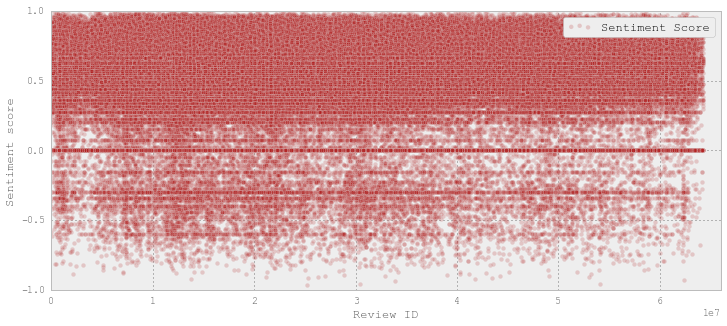
\includegraphics[height=0.24\textheight]{sentiment}
	\caption{Sentiment scores of each sentence of reviews in the dataset}
	\label{fig:sent}
\end{figure}
The sentiment scores are also grouped by accommodation features and for each of them its seen the distribution of these scores. By comparing these distributions to each other and to the overall sentiment scores, it is noticed that the more the feature is mentioned the more similar the distribution is with the overall sentiment pattern. However, small differences are recognized for each feature, for example the values of feature \textit{cleanliness} have a tendency to be mostly positive and grouped between 0.3-0.5 or 0.7-0.9. These patterns of distribution can all be found in Appendix I.

An interesting point of view is the analysis of what features are most mentioned in proportion with the number of comments in the listing. This analysis is done in three levels: sentence level, review level and listing level. For all the three levels, we can clearly see that \textit{location} is the most mentioned feature by reviewers of Airbnb and \textit{check-in} is the least mentioned one. From this comparison we can also indicate that the frequency of mentioning features is more accurate in review level, as in the first case the number of sentences is very high which makes the percentage be under-estimated. On the other hand, in listing level it would take at least one sentence to indicate that the feature is mentioned in the listing, no matter if at one listing is mentioned 100 times, which can cause over-estimation.
\begin{figure}[h!]
\centering
	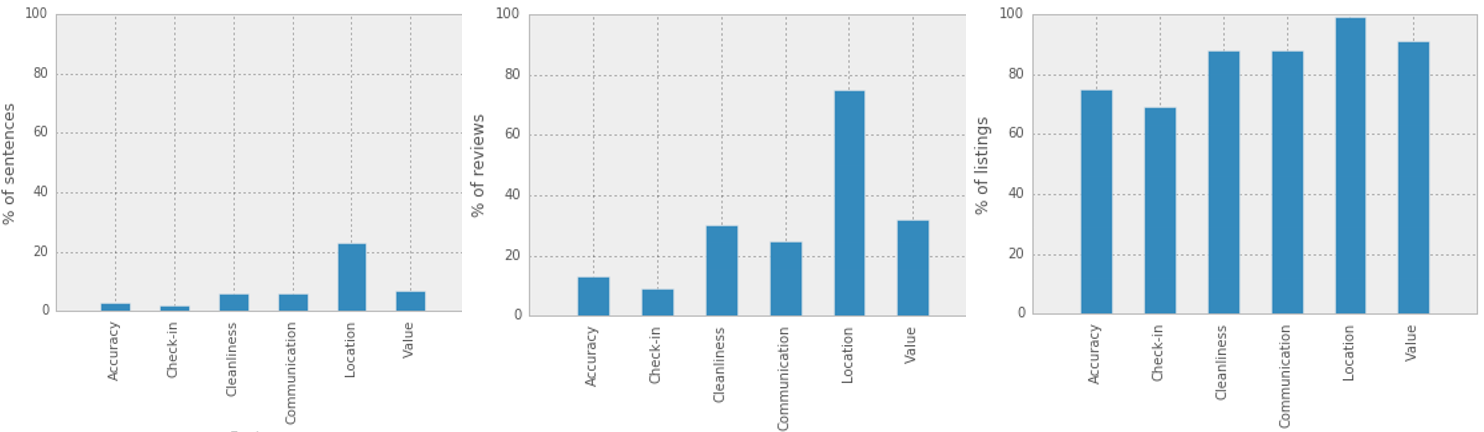
\includegraphics[height=0.2\textheight]{feature_mentioned}
	\caption{Percentage of sentences, reviews and listings where the features are mentioned}
	\label{fig:fea}
\end{figure} 
\begin{figure}[h!]
	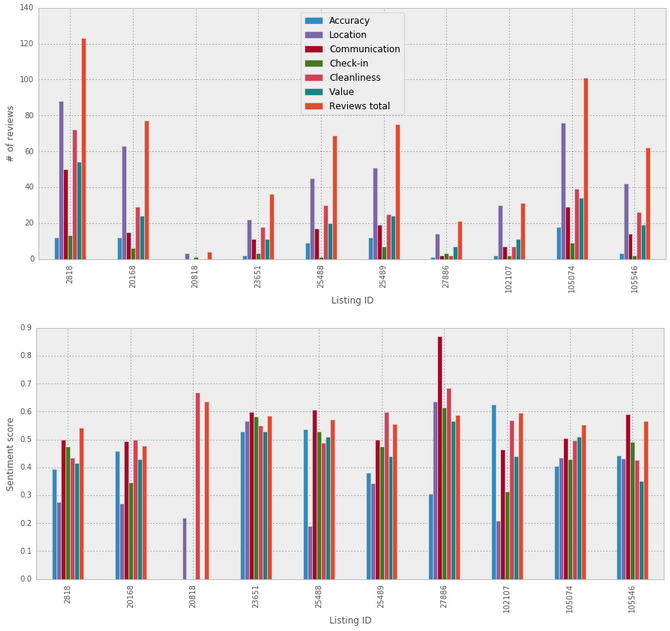
\includegraphics[height=0.57\textheight]{features_sentiment}
	\caption{Features mentioned in review level per each listing and their sentiment}
	\label{fig:feasent}
\end{figure}
Following this logic, Figure \ref{fig:feasent} represents for each listing the number of reviews which mention the features and it compares it to the overall number of reviews. In this way, we would prefer to choose listings where we have many reviews for a certain features i.e. \textit{location} compared to the overall number of reviews in order for the sentiment score to be more reliable.  %calculation of overall negative scores per feature, by which we can find out which listing has less negative comments in proportion to the number of comments in total.
For each of the listings the compound sentiment scores over a certain feature are easily calculated. The second part of Figure \ref{fig:feasent} shows for the same ten listings the compound sentiment scores of each feature and the compound sentiment. In this way, the sentiment scores can be compared with the number of reviews. From the Figure we can see that for the listing with ID 22886, even though it has the highest sentiment score on \textit{communication}, it is reviewed by only a very few people, compared to the other listings. This result means that the sentiment score of the first listing would be more reliable than the one with a few reviewers but a good sentiment score. In this case each customer would have to make an individual choice for which listing they would go by considering both the number of reviews on a certain feature and their sentiment. 

Another aspect of analysis from the generated sentiment scores is their comparison with the Airbnb quantitative data. In the Airbnb feedback system, the customers can see the number of reviews for a listing, the overall average rating after the first three reviews and the average rating of the six specific features: \textit{accuracy, check-in, cleanliness, communication, location, value}. These ratings are compared to the ratings generated by the pipeline by converting the sentiment scores [-1;1] in the scale 1 to 5 stars. From the analysis we can notice that the overall ratings of generated from the pipeline are quite similar to the ratings in the Airbnb system. 
\begin{figure}[h!]
\centering
	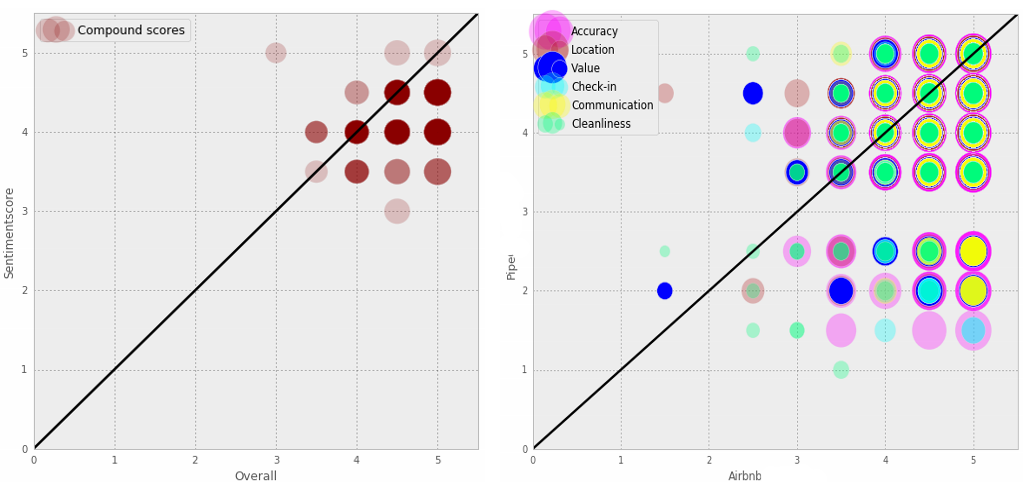
\includegraphics[height=0.33\textheight]{overall_features}
	\caption{Comparison of overall and features rating distribution}
	\label{fig:ovfea}
    	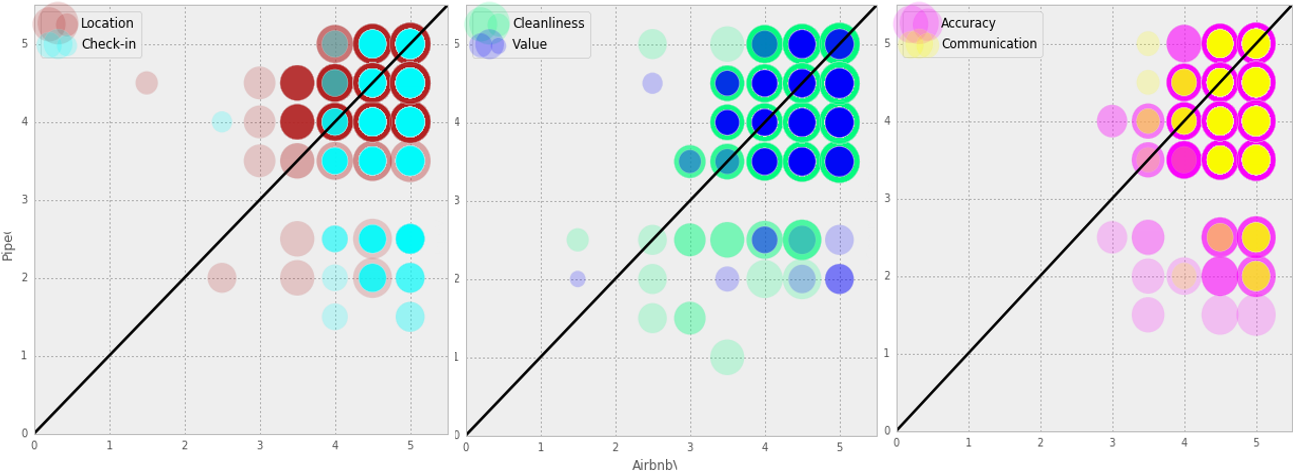
\includegraphics[height=0.25\textheight]{features_distribution}
	\caption{Features rating distribution detailed}
	\label{fig:fea}
\end{figure}

It is obvious from Figure \ref{fig:ovfea} a) that there is no listing with negative sentiment, lower than 3 stars, both in Airbnb system and the pipeline results. Furthermore there is a tendency of Airbnb ratings to be higher than the ratings generated from the text feedback, concretely in 89.7\% of the cases, consisting in a difference of half a star in 50.6\% of cases, one star in 38.7\% of cases and only 0.3\% of difference more than one star. The standard error of the mean (SEM) between the pipeline sample and Airbnb is 0.0096 which indicates a precise estimation of compound ratings. These results prove the precision of the pipeline in predicting the overall rating of the listings based on text feedback and in the same time indicate a factor of reducing bias in the Airbnb system, as suggested by \cite{fradkin2016bias}. The only outlier for the compound ratings of the pipeline compared to Airbnb is a case where the sentiment predicted for a listing is 5 stars, when the Airbnb system assigns only 3. Since this case case is isolated and occurs only once, we have considered it in the range of errors of the pipeline precision. 

Similarly in feature level we can also see that most of the rating values of Airbnb and pipeline fall in the upper corner of the quadrant, however it is obvious the presence of a big number of outliers. The ones that interest us are the values for which the pipeline estimates negative ratings (lower than 3) but in Airbnb those features are rated with the maximum number of stars. From Figure \ref{fig:ovfea} b) and its detailed version Figure \ref{fig:fea}, we can notice that this phenomenon is present at every feature, but most likely for \textit{Check-in, Communication } and \textit{Accuracy}. The findings are also supported by the standard error of the mean (SEM), which is higher for these three features and the lowest for \textit{location} and \textit{communication} respectively 0.01 and 0.008. These findings align with the fact that \textit{location} and \textit{cleanliness} resulted to be the most mentioned features in the reviews, therefore the higher the number of cases in the sample the bigger the precision. Furthermore, from the evaluation of the pipeline we saw that feature extraction is most accurate and precise for \textit{cleanliness} therefore the results are more reliable. On the other hand, for \textit{check-in} the evaluation of pipeline suggests that half of the cases mentioning this feature are missed by the pipeline. Therefore, the explanation of the outliers can lay between the accuracy of the pipeline on extracting features from the text and the real frequency of features mentioned in reviews. Thus, the better the feature identification from pipeline and the higher the feature is mentioned in reviews, the smaller is the number of outliers in distribution of pipeline generated ratings per feature compared to Airbnb and overall ratings.

Another aspect that the analysis of text feedback can be used is for checking the number of times when the host has canceled the reservation. Every time that the reservation is canceled an automatic message is posted in the text feedback space as a review by the guest-to-be. The occurrence of these types of messages can be check for all the listings and from the analysis we could retrieve the listings which have the highest probability of canceling. It was noticed that in a rare case the number of cancellations reached 27, however the mean number of cancellation would be 1.7 per listing. In total there are 32.8\% of the listings which have canceled at least once the reservation, meaning that the customers would have to pay attention to these cases in order to let their plans spoiled.

Many other insights can be drawn from the analysis of the sentiment scores and features extracted, which are similar to the analysis of quantitative data as we deal only with discrete sentiment scores. These results showed the alignment between the quantitative data of Airbnb as star ratings with the output of the pipeline. Furthermore, they showed that the text feedback can reveal hidden knowledge which can not be obtained only by analyzing the ratings in the feedback system. The analysis involves both the customer and business perspective therefore it is seen as an interesting aspect to explore further than this research.